% \section{The WebAnno interface}
% - show annotation panel
% - show sidepanel
% - clear
% - Explain existing annotations: What came before

\section{Sentiment Expression}
\label{sec:sentimentexpressiondefinition}
Sentiment can be both explicit expressions of opinion in the text as well as descriptions of events or situations with a specific connotation that evokes a certain sentiment.
\\\\
\noindent
A \textbf{Sentiment Expression is (sequence of) word(s)} that
\begin{enumerate}[label=\alph*), leftmargin=*]
    \item \textbf{affects \hyperref[sec:sentimentdef]{investor sentiment}} towards a company, market, stock, asset or person. e.g., \textit{``fall in stock price'', ``decline in sales and revenue'', ``increase in performance'', ``positive return on investment'', ``growing consumer interest''}.
    \item expresses positive or negative \textbf{opinion}. e.g. \textit{``strong performance'', ``being bad for'', ``fall from grace''}.
\end{enumerate}
\noindent
Look for words that stand out in conveying the content that would inform an investor’s opinion on a stock, person, market. Are there words that will influence the opinion of a potential investor?
It is likely that there are \textbf{multiple Sentiment Expressions per sentence}.
\textbf{Some Sentiment Expressions are already annotated as pre-existing Event annotations}.
You do not have to annotate new sentiment expressions on top of these Events.\\\\
\noindent
\textcolor{BrickRed}{NOTE: Avoid annotating full clauses: often annotating only the verb or the noun is sufficient for capturing the core meaning of the sentiment. Avoid annotating the companies, markets, stocks, assets or persons involved in the Sentiment Expression. Keep the \textbf{number of words as small as possible}.}

\begin{figure}[h]
    \centering
    
\includegraphics[width=\textwidth]{img/cost03s11 general example.png}
    \caption*{$\rightarrow$ \textbf{Sentiment Expression}: ``positively impacted'' is an example of a positive Sentiment Expression. ``tax benefit'' is a pre-existing Event annotation that is also a Sentiment Expression.}
    \label{fig:se_ex1}
\end{figure}

\begin{figure}[h]
    \centering
    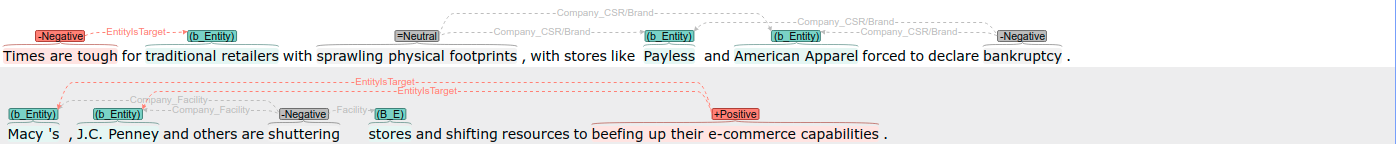
\includegraphics[width=\textwidth]{img/amzn00s9-10 negative event example.png}
    \caption*{$\rightarrow$ \textbf{Sentiment Expression}: ``Times are tough'' is a negative Sentiment Expression, ``beefing up their e-commerce capabilities'' is a Positive Sentiment Expression, ``sprawling physical footprints'' is a neutral Sentiment Expression as a pre-existing Event annotation, ``bankruptcy'' is a negative Sentiment Expressions  as a pre-existing Event annotation, ``shuttering'' is a negative Sentiment Expression as a pre-existing Event annotation.}
    \label{fig:se_ex2}
\end{figure}

\noindent
\textcolor{BrickRed}{NOTE: \textbf{Relevancy} of sentiment expressions: since we are primarily interested in company-specific investor sentiment you should only annotate new \textbf{sentiment expressions that are relevant to a company}. Sentiment expressions about companies, company-specific assets, reports or metrics, and people, infrastructure or subsidiaries related to a company are relevant should be annotated. Irrelevant background information about products, locations or other details that do not \textbf{affect an investors opinion of a company} should not be annotated.}

\subsection{Sentiment Polarity}
\label{sec:polaritydefinition}
Sentiment Expressions always have a positive, negative or neutral Polarity.
Polarity is the emotional opinion value of the Sentiment Expression.
Positive polarity signals an optimistic, desirable, pleasant or favourable disposition, while Negative polarity signals pessimistic, undesirable, or unpleasant attitudes.

For our definition of common-sense investor sentiment, positive polarity are Sentiment Expressions that express a positive attitude towards a business entity directly or are indirectly good for an investor looking to invest in that business entity. Positive polarity Sentiment Expressions then signal all things that increase the likelihood of return on profit when investing in the target business entity.
Negative polarity does the opposite: negative polarity Sentiment Expressions decrease the likelihood of a return on profit when investing in the target.

Besides positive and negative polarity, we also annotate Neutral polarity making three polarity values in total:

\begin{enumerate}[label=\alph*), leftmargin=*] % insert figure here and explain in more detail
    \item \textbf{Positive}: an event, opinion or situation that increases the likelihood of a return on investment.
    Positive Sentiment Expressions directly or indirectly improve the attitude of a potential investor towards the target.
    \item \textbf{Negative}: an event, opinion or situation that increases the likelihood of a loss on investment.
    Negative Sentiment Expressions directly or indirectly diminish the attitude of a potential investor towards the target.
    \item \textbf{Neutral}: an event, opinion or situation has no clear positive or negative polarity.
    This happens when a) it is unclear how the Sentiment Expression affects a potential investor's attitude or b) the annotator cannot identify a clearly positive or negative polarity.
    When doubting between Positive/Negative and Neutral sentiment, annotators should prefer to assign Positive/Negative.
    % \item \textbf{Conflict}: the sentiment of an event, opinion or situation depends on the point of view of the reader or is highly debatable.
    % Personal preferences, political bias, or sentiment highly dependent on context or perspectives outside of the article are typical cases.
    % Do not confuse this with Neutral sentiment: there should be a clear conflict of point of view, not an unclear sentiment.
     % TODO Make this a double tagging rule instead of CONFLICT and DISCUSS in DIFFICULT CASES SECTION
\end{enumerate}

\begin{figure}[h]
\captionsetup[subfigure]{labelformat=empty}
\begin{subfloat}
    \centering
    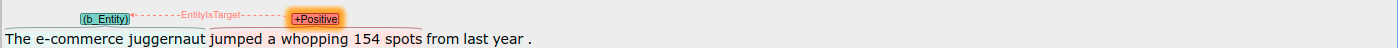
\includegraphics[width=\textwidth]{img/amzn00-s04 pos example.png}
    \caption*{$\rightarrow$ \textbf{Positive}: New Sentiment Expression ``jumped a whopping 154 spots [in ranking]'' is Positive for the e-commerce giant Amazon.}
\end{subfloat}

\begin{subfloat}
    \centering
    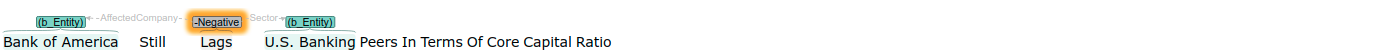
\includegraphics[width=\textwidth]{img/bac02s01 negative example.png}
    \caption*{$\rightarrow$ \textbf{Negative}: Pre-existing Event annotation ``Lags'' is Negative for ``Bank of America''.}
\end{subfloat}

\begin{subfloat}
    \centering
    
\includegraphics[width=\textwidth]{img/bac02s04 neutral example.png}
    \caption*{$\rightarrow$ \textbf{Neutral}: Pre-existing Event annotation ``CET1 Buffer'' is Neutral for ``Bank of America'' as it is not clearly bad or good.}
\end{subfloat}

% % TODO FIND A BETTER CONFLICT EXAMPLE BECAUSE THIS ONE IS NOT IT
% \begin{subfloat}
%     \centering
%     
\includegraphics[width=\textwidth]{img/amzn00s01 conflict example.png}
%     \caption*{$\rightarrow$ \textbf{Conflict}: Pre-existing Event annotation ``Closing in'' is good for ``Amazon'' and ``Alibaba'', but bad for ``Walmart''. Due to this conflict inherent in the event we annotate Conflict polarity.}
% \end{subfloat}
\end{figure}

\begin{wrapfigure}[4]{R}{0.3\textwidth}
    \centering
    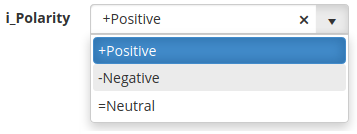
\includegraphics[width=0.3\textwidth]{img/polarityui.png}
    \vspace{-10pt}
    \label{fig:polarityui}
\end{wrapfigure}

\noindent
\textcolor{Blue}{Annotate Polarity in the WebAnno interface:
1) Select the Sentiment Expression or pre-existing Event in the annotation panel by double-clicking.
2) Select \texttt{Positive}, \texttt{Negative}, or \texttt{Neutral} from the drop-down menu next to \texttt{f\_Polarity} in the side panel.}

\subsection{Sentiment Uncertainty}
\label{sec:uncertaintydefinition}
Most sentiment expressions are asserted by the news article author as lacking any uncertainty.
However, some Sentiment Expressions have a degree of uncertainty: these are represented by the author as probable, possible or likely sentiment expressions and improbably, impossible or unlikely sentiment expressions.
The author indicates it is a \textbf{possibility, probability or likelihood that the event takes place or does not take place}.
The Uncertainty label also includes cases in which the author signals that he does not know the certainty level or does not commit to asserting a fact.

Uncertainty can be realized by uncertainty markers such as verbal auxiliaries (must, may), adverbials (probably, possibly, presumably), and adjectives (likely, possible).
In many cases, uncertainty will be conveyed by verbs near the sentiment expression: "seem", "think", "want", "wish", "hope", "speculate", "propose", \annexe{The company \uline{wants} to \anntrg{fire} its factory line workforce.}

\begin{figure}[h]
    \centering
    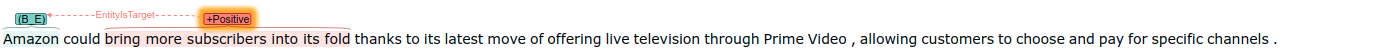
\includegraphics[width=\textwidth]{img/amzn04s31 uncertain example.png}
    \caption*{$\rightarrow$ \textbf{Uncertain}: Sentiment Expression ``bring more subscribers into its fold'' is uncertain due to the auxiliary verb ``could''.}
    \label{fig:unc_ex1}
\end{figure}

\noindent
\textcolor{BrickRed}{NOTE: Uncertainty only has to be annotated on new Sentiment Expressions. Pre-existing Events already have Uncertainty annotated by previous annotators.}\\

\begin{wrapfigure}{R}{0.2\textwidth}
    \centering
    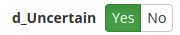
\includegraphics[width=0.2\textwidth]{img/uncertainui.png}
    \label{fig:uncertainui}
\end{wrapfigure}

\noindent
\textcolor{Blue}{Annotate Uncertainty in the WebAnno interface:
1) Select the Sentiment Expression in the annotation panel by double-clicking.
2) Click the toggle in the side panel next to \texttt{e\_Uncertain} if the sentiment has Uncertainty otherwise do nothing. The toggle should turn from red \texttt{No} to green \texttt{Yes}.}


\subsection{Sentiment Negation}
\label{sec:negationdefinition}

Usually, the sentiment expressed by the Sentiment Expression is affirmative and asserted, meaning that it is being represented as being true or as something that will happen/has happened.
However, a Sentiment Expression can also be negated in its context.
\textbf{A negative form expresses the falsity of the opinion, event or situation expressed}.
It communicates the opposite meaning of the opinion, event or situation.
This is typically realized by ``not'', ``-n't'', ``no'', ``noone'', ``nowhere'' or other negative forms.\\

\noindent
\textcolor{BrickRed}{NOTE: The negation word should not be tagged as part of the Sentiment Expression.
Because of this, the Polarity of the sentiment should be opposite of its meaning in the full negated context:}\\

\begin{figure}[h]
    \centering
    
\includegraphics[width=\textwidth]{img/amzn04s34 negated negative sentiment.png}
    \caption*{$\rightarrow$ \textbf{Negated}: we annotate ``run out of steam'' and not ``is not going to run out of steam'' as the Sentiment Expression: we do not include the negation word ``not''. While the meaning of the whole sentence is Positive, ``run out of steam'' is tagged as Negative because the phrase on its own is Negative.}
    \label{fig:neg_ex1}
\end{figure}

\begin{figure}[h]
    \centering
    
\includegraphics[width=\textwidth]{img/cost02s02 new sentiment negative uncertain.png}
    \caption*{$\rightarrow$ \textbf{Negated + Uncertain}: ``slowing down'' is negated by ``doesn't'' and uncertainty is added by ``seem''. While the meaning of the whole sentence is Positive, ``slowing down'' is tagged as Negative because on its own without the negation of ``doesn't'' it signals Negative polarity.}
    \label{fig:neg_ex2}
\end{figure}

\noindent
\textcolor{BrickRed}{NOTE: Negation only has to be annotated on new Sentiment Expressions. Pre-existing Events already have Negation annotated by previous annotators.}\\

\begin{wrapfigure}{l}{0.2\textwidth}
    \centering
    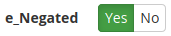
\includegraphics[width=0.2\textwidth]{img/negationui.png}
    \label{fig:negationui}
\end{wrapfigure}

\noindent
\textcolor{Blue}{Annotate Negation in the WebAnno interface:
1) Select the Sentiment Expression in the annotation panel by double-clicking.
2) Click the toggle next to \texttt{e\_Negated} if the sentiment is negated otherwise do nothing. The toggle should turn from red No to green Yes.}

\section{Events (Pre-existing annotation)}
\label{sec:eventdefinition}
When you open a document in the WebAnno interface, pre-existing annotations will be present in the text that were made in a previous annotation task.
You will add your own sentiment annotations on top of these annotations.
There are two pre-existing annotation categories: Events and Entities.
Here we discuss Events briefly:\\
\eventcolor Event annotation with label \texttt{a\_Event} and label \texttt{d\_EventPart} for unconnected words that are part of the event.

\begin{figure}[!htb]
    \centering
    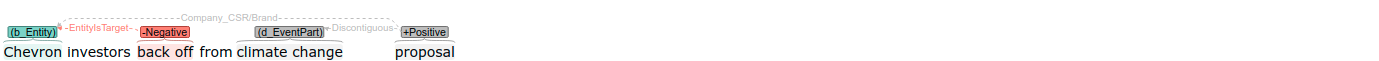
\includegraphics[width=\textwidth]{img/cvx00s01 event part.png}
    \caption*{$\rightarrow$ \textbf{Split Event+EventPart}: ``climate change proposal'' is split in two labels but should be read as one Event.}
\end{figure}

Events denote real-world actions, changes and situations which are relevant to economic news.
These events come from a prescribed set of 18 categories such as ``Investment'', ``Dividend'', ``Security Value'', ``Mergers \& Acquisitions'', etc. 
You should ignore the types of these events, however note that potentially relevant Events not belonging to these 18 types were not annotated.
This means that you will have to pay attention to relevant news events that invoke sentiment and annotate them as new Sentiment Expressions.\\

\noindent
\textcolor{BrickRed}{NOTE: Often pre-existing Event annotations will not include all words that capture the full sentiment.
In that case, we simply assign the polarity on the event as if it was part of a full Sentiment Expression.}
\begin{figure}[h]
    \centering
    
\includegraphics[width=\textwidth]{img/fb03 incomplemte event trigger example.png}
    \caption*{$\rightarrow$ \textbf{Event}: ``terrorism'' is a pre-existing Event annotation. While the full Sentiment Expression would be ``cracking down on terrorism'', indicating Positive opinion, you only have to assign the polarity on the pre-existing Event, not on the whole phrase.}
\end{figure}

Annotators assign all pre-existing Events a polarity value of Positive, Negative, or Neutral taking into account the definition of events above.
Annotators should take into account the \textbf{whole context of the event when determining the event polarity}.
This means that the framing of the event and its participants are important. However, an \textbf{exception are Negated events which should ignore the negation context} when annotating polarity in the same manner as new Sentiment Expressions. Negation has already been tagged on these Events as a pre-existing annotation.\\

\noindent
\textcolor{BrickRed}{NOTE: When multiple Events are annotated in the same location. Do not forget to determine polarity for all Events taking into account the different Entities involved in the different Events. If they have the same Entities, annotate the same polarity on all events.}
\begin{figure}[h]
    \centering
    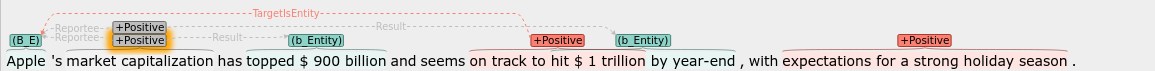
\includegraphics[width=\textwidth]{img/aapl15 s04 two events in same place.png}
    \caption*{$\rightarrow$ \textbf{Event}: ``market capitalization'' has two pre-existing Event annotations. The first links to the Entity ``topped \$ 900 billion'', indicating Positive opinion. The second event links to Entity ``hit \$ 1 trillion by year-end'' which is also Positive. Polarity for both events is annotated.}
\end{figure}

\section{Entities (Pre-existing annotation)}
\label{sec:entitydefinition}
\entitycolor Entity annotations with label \texttt{b\_Entity}.
    
These are the central participants involved in the event.
Entities play a typical role in the Event to which they are linked.
They are often companies, persons, assets or monetary amounts.
This role label is visible in the annotation interface on the link, but should be ignored for our purposes.
The existing entity annotations can be realized as pronouns (``it'', ``its'', ``he(r)''. ``they'', ``we'') or non-specific descriptions (``the company'', ``the bank'', ``the tech giant'').
If you annotate new entities as targets (cf. \ref{sec:entitydefinition}) you should not annotate pronouns but the nearest specific mention of the entity.

You will also make new Entity annotations when they are the target of a Sentiment Expression.

\begin{figure}[h]
    \centering
    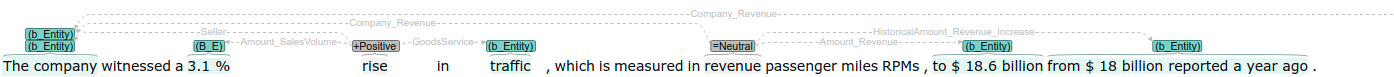
\includegraphics[width=\textwidth]{img/aal00s03 entities example.png}
    \caption*{$\rightarrow$ \textbf{Entity}: Several \entitycolor pre-existing Entity annotations as participants in the Event annotations.}
    \label{fig:ent_ex1}
\end{figure}

\section{Target}
\label{sec:targetdefinition}
The target of a sentiment is the company, person, product, asset, entity, etc. about which the sentiment is expressed.
A person always expresses an opinion about some topic and that topic is the target.
The target is the entity about which a potential investor forms his opinion.
One Sentiment Expression can have multiple targets and all targets should be tagged.

\noindent
In our annotation task we have three categories of targets:
\begin{enumerate}[label=\alph*), leftmargin=*]
    \item \textbf{New target entity}: the target entity is expressed by words on which NO Entity or Event annotation exists.
    \begin{figure}[!htb]
    \centering
    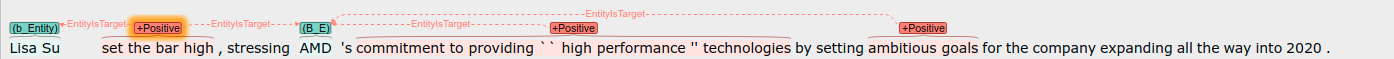
\includegraphics[width=\textwidth]{img/amd02s08 new entity.png}
    \caption*{$\rightarrow$ This sentence had no pre-existing annotations. New target Entity annotations must be made for ``Lisa Su'' target of Sentiment Expression ``set the bar high'', ``AMD'' target of ``commitment to providing...'' and ``ambitious goals''.}
\end{figure}

    \item \textbf{Existing Entity}: the target entity is expressed by words on which a \entitycolor Entity annotation exists.
    \begin{figure}[!htb]
    \centering
    
\includegraphics[width=\textwidth]{img/aal02s11 entity .png}
    \caption*{$\rightarrow$ Sentiment Expression ``on time'' targets pre-existing Entity ``AA''.}
\end{figure}
    
    \item \textbf{Existing Event}: the target is an event on which a \eventcolor Event annotation exists.
    \begin{figure}[!htb]
    \centering
    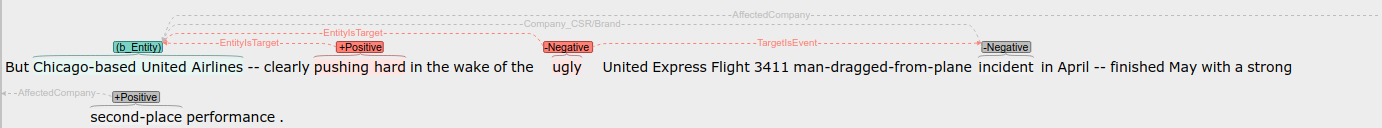
\includegraphics[width=\textwidth]{img/aal02s06 entity target example.png}
    \caption*{$\rightarrow$ ``ugly'' has two targets: pre-existing Event ``incident'' and pre-existing Entity ``Chicago-based United Airlines''.}
\end{figure}
\end{enumerate}

You will have to annotate new targets and link the Sentiment Expression to existing Event or Entity targets.
Keep the \textbf{word sequence of New target annotations as small as possible} to capture the core meaning of the target.

\newpage
\noindent
\textcolor{BrickRed}{NOTE: \textbf{Target-dependent polarity}: The \textbf{sentiment polarity of an expression changes depending on the target}.
This usually happens when a contrasting comparison is made between two companies.
In that case, annotate two different Sentiment Expressions with different polarity and targets in the same place.\\
An existing Event can also have different polarity for different participants.
In this case, annotate the Event itself as Neutral because its Polarity is ambiguous and make new Sentiment Expressions exactly on top of the existing Event expression with the Polarity corresponding to each Target.}

\begin{figure}[!ht]
    \centering
    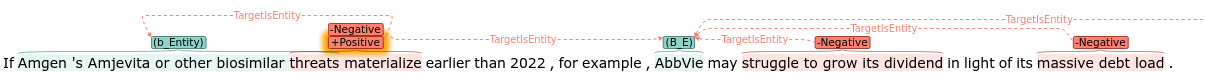
\includegraphics[width=\textwidth]{img/abbv07 s31 target dependent new sentiment example.png}
    \caption*{$\rightarrow$ \textbf{Target-dependent polarity double tagging}: New Sentiment Expression ``threats materialized'' is positive for the target ``Amgen's Amjevita or other biosimilar threats'', but negative for ``AbbVie'' so we annotate one positive and one negative Sentiment Expression in the same place.}
\end{figure}

\begin{figure}[!ht]
    \centering
    
\includegraphics[width=\textwidth]{img/amz00 s01 target dependent polarity double tagging on event.png}
    \caption*{$\rightarrow$ \textbf{Target-dependent polarity double with existing Event}: Existing Event ``Closing in'' is tagged as ``Neutral'' because the event itself is ambiguous. 
    Two new Sentiment Expressions are made exactly in the same place as ``Closing in'': One Positive for targets ``Amazon'' and ``Alibaba''and another Negative for ``Walmart''.}
\end{figure}


% ISSUES TO BE RESOLVED: if one event combines a positive or negative effect on different participants
% Possible solution:
% - Annotate Conflict as polarity
% - 
